%pbssm
\documentclass[../../main/main.tex]{subfiles}




\begin{document}
\title{Patrol Base Operations as Secure State Machines}


%%%%%%%%%%%%%%%%%%%%% Chapter PB SSM %%%%%%%%%%%%%%%
\chapter{Patrol Base Operations as Secure State Machines} \label{chp:pbssm}
The hierarchy of secure state machines (\glsentryshortpl{ssm}) consists of many \glsentryshortpl{ssm}.  Ten of these \glsentryshort{ssm} are verified in \glsentryshort{hol}.  Many of these \glsentryshortpl{ssm} are similar.  Thus, a sampling of representative \glsentryshortpl{ssm} is described in this section.  All \glsentryshortpl{ssm} can be found in the appendices starting with appendix \ref{app:ssms}.  They are also contained in the MasterThesis/HOL/ folders.

      %%%%%%%%%%%%%%%%%%% Section ssmPB %%%%%%%%%%%%%
\section{ssmPB: A Typical Example from the Hierarchy}\label{sec:ssmpb}
ssmPB is the top level \glsentryshort{ssm}.  It is an example of a typical one-principal \glsentryshort{ssm}.

\subsection{Principals}
\subsection{States}
\subsection{Commands}
\subsection{Next-State Function}
\subsection{Next-Output Function}
\subsection{Authentication}
\subsection{Authorization}
\subsection{Proved Theorems}
\subsubsection{Platoon Leader Is Trusted on plCommands}


     
      %%%%%%%%%%%%%%%%%%% Multiple Principles %%%%%%%%%%%%%
\section{ssmConductORP: Multiple Principals}
ssmConductORP is an example of a \glsentryshort{ssm} with more than one principal authorized to execute transitions among states.

\subsection{Principals}
\subsection{States}
\subsection{Commands}
\subsection{Next-State Function}
\subsection{Next-Output Function}
\subsection{Authentication}
\subsection{Authorization}
\subsection{Proved Theorems}



      %%%%%%%%%%%%%%%%%%% ssmPlanPB %%%%%%%%%%%%%%%%
\section{ssmPlanPB: Non-sequential Transitions}
The ssmPlanPB \glsentryshort{ssm} is one of the first \glsentryshortpl{ssm}\footnote{This is only partially true.  The first \glsentryshort{ssm} was ssmPB.  But, upon working with the \glsentryshort{ssm} in this section, the parametrizable ssm needed to updated to accommodate multiple input statements.  ssmPlanPB was the first \glsentryshort{ssm} used with this new parametrizable ssm.  All other \glsentryshortpl{ssm} were redone with the updated parametrizable ssm.}. It is the only \glsentryshort{ssm} that is not integrated with the Omni principal.  But, it is also the only \glsentryshort{ssm} that uses a non-sequential progression through states.  Figure \ref{ssmPlanPBDiagram2} is a diagram of this \glsentryshort{ssm}.

\begin{figure}[h!]
\centering
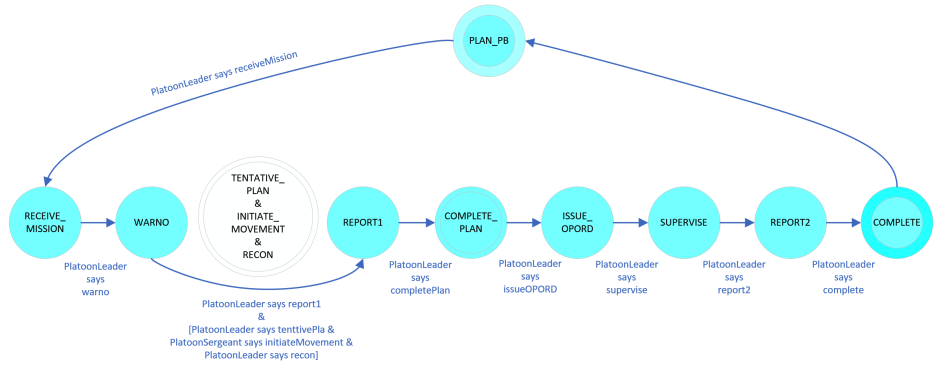
\includegraphics[width=\textwidth]{../figures/ssmPlanPBDiagram}
\caption{\label{ssmPlanPBDiagram2} Horizontal slice: PlanPB diagram.}
\end{figure}

The three non-sequential states are hidden in the white circle in the diagram.  They are TENTATIVE_PLAN, INITIATE_MOVEMENT, and RECON. These three states may be completed in any order, but all three must be completed before progressing to the next state REPORT1.  

To handle this, the three non-sequential states are combined into a "virtual state."  This state does not exist.  But, completion of these states must preceded transition from the WARNO state to the REPORT1 state.  Completion is indicated by the following three \glsentryshort{acl} statements
\[\text{\textit{PlatoonLeader says tentativePlan}}\]
\[\text{\textit{PlatoonSergeant says initiateMovement}}\]
\[\text{\textit{PlatoonLeader says recon}}\]


when combined with a request from the PlatoonLeader to transition to the REPORT1 state, the input for this transition is an input list with the four statements
\[\text{\textit{PlatoonLeader says tentativePlan}  }\]
\[\text{\textit{PlatoonSergeant says initiateMovement}  }\]
\[\text{\textit{PlatoonLeader says recon}}\]
\[\text{\textit{PlatoonLeader says report1}}\]

The security policy handles this with the following implication
\[\text{\textit{tentativePlan} andf  }\]
\[\text{\textit{initiateMovement} andf  }\]
\[\text{\textit{recon} impf}\]
\[\text{\textit{PlatoonLeader controls recon}}\]

The remaining details of this implementation follow.
\subsection{Principals}
The planning phase \glsentryshort{ssm} has two principals: PlatoonLeader and PlatoonSergeant.  These are defined in the \HOLFreeVar{stateRole} datatype.

\HOLFreeVar{stateRole} = \HOLConst{PlatoonLeader} \HOLTokenBar{} \HOLConst{PlatoonSergeant}

\subsection{States}
There are 12 states.  But, TENTATIVE_PLAN, INITIATE_MOVEMENT, and RECON are virtual states and not used in the next-state and next-output functions.

\begin{tabbing}
\parskip=8pt
\HOLFreeVar{slState} = \=\HOLConst{PLAN_PB} \\
				\>\HOLTokenBar{} \HOLConst{RECEIVE_MISSION} \\
				\>\HOLTokenBar{} \HOLConst{WARNO} \\
				\>\HOLTokenBar{} \HOLConst{TENTATIVE_PLAN}\\
        				\>\HOLTokenBar{} \HOLConst{INITIATE_MOVEMENT} \\
				\>\HOLTokenBar{} \HOLConst{RECON} \\
				\>\HOLTokenBar{} \HOLConst{REPORT1} \\
				\>\HOLTokenBar{} \HOLConst{COMPLETE_PLAN}\\
        				\>\HOLTokenBar{} \HOLConst{OPOID} \\
				\>\HOLTokenBar{} \HOLConst{SUPERVISE} \\
				\>\HOLTokenBar{} \HOLConst{REPORT2} \\
				\>\HOLTokenBar{} \HOLConst{COMPLETE}
\parskip=18pt
\end{tabbing}

\subsection{Commands}
The slCommand datatype for this \glsentryshort{ssm} is defined below.

\HOLFreeVar{slCommand} = \HOLConst{PL} \HOLTyOp{plCommand} \HOLTokenBar{} \HOLConst{PSG} \HOLTyOp{psgCommand}

The two datatypes for plCommand and psgCommand represent the PlatoonLeader and PlatoonSergeant commands, respectively. These are defined below.

\begin{tabbing}
\parskip=8pt
\HOLFreeVar{plCommand} = \=\HOLConst{receiveMission} \\
					     \>\HOLTokenBar{} \HOLConst{warno} \\
					     \>\HOLTokenBar{} \HOLConst{tentativePlan} \\
					     \>\HOLTokenBar{} \HOLConst{recon}\\
          				     \>\HOLTokenBar{} \HOLConst{report1} \\
				     	     \>\HOLTokenBar{} \HOLConst{completePlan} \\
					     \>\HOLTokenBar{} \HOLConst{opoid} \\
					     \>\HOLTokenBar{} \HOLConst{supervise} \\
					     \>\HOLTokenBar{} \HOLConst{report2}\\
          				     \>\HOLTokenBar{} \HOLConst{complete} \\
				     	     \>\HOLTokenBar{} \HOLConst{plIncomplete} \\
					     \>\HOLTokenBar{} \HOLConst{invalidPlCommand}
\parskip=18pt
\end{tabbing}

\begin{tabbing}
\parskip=8pt
\HOLFreeVar{psgCommand} = \=\HOLConst{initiateMovement} \\
						\>\HOLTokenBar{} \HOLConst{psgIncomplete}\\
           					\>\HOLTokenBar{} \HOLConst{invalidPsgCommand}
\parskip=18pt
\end{tabbing}

Providing each principal with her own set of commands simplifies the authentication and authorization functions.
\subsection{Output}
There are 14 outputs.  But, PlanPB, TentativePlan, InitiateMovement, and Recon are not used in the next-output function.  The unAuthorized output is returned for discarded commands.  The unAuthenticated output is returned for discarded commands.

\begin{tabbing}
\parskip=8pt
\HOLFreeVar{slOutput} =  \=\HOLConst{PlanPB} \\
					\>\HOLTokenBar{} \HOLConst{ReceiveMission} \\
					\>\HOLTokenBar{} \HOLConst{Warno} \\
					\>\HOLTokenBar{} \HOLConst{TentativePlan}\\
         				\>\HOLTokenBar{} \HOLConst{InitiateMovement} \\
					\>\HOLTokenBar{} \HOLConst{Recon} \\
					\>\HOLTokenBar{} \HOLConst{Report1} \\
					\>\HOLTokenBar{} \HOLConst{CompletePlan}\\
         				\>\HOLTokenBar{} \HOLConst{Opoid} \\
					\>\HOLTokenBar{} \HOLConst{Supervise} \\
					\>\HOLTokenBar{} \HOLConst{Report2} \\
					\>\HOLTokenBar{} \HOLConst{Complete}\\
         				\>\HOLTokenBar{} \HOLConst{unAuthenticated} \\
					\>\HOLTokenBar{} \HOLConst{unAuthorized}
\parskip=18pt
\end{tabbing}

\subsection{Next-State Function}
\begin{tabbing}
\parskip=8pt
\HOLTokenTurnstile{} \\
\hspace{0.3cm}(\HOLConst{planPBNS} \HOLConst{WARNO} (\HOLConst{exec} \HOLFreeVar{x}) \HOLSymConst{=}\\
\hspace{0.5cm} \HOLKeyword{if}\\
\hspace{0.9cm}(\HOLConst{getRecon} \HOLFreeVar{x} \hspace{1.8cm}\=\HOLSymConst{=} [\HOLConst{SOME} (\HOLConst{SLc} (\HOLConst{PL} \HOLConst{recon}))]) \HOLSymConst{\HOLTokenConj{}}\\
\hspace{0.9cm}(\HOLConst{getTenativePlan} \HOLFreeVar{x} \>\HOLSymConst{=} [\HOLConst{SOME} (\HOLConst{SLc} (\HOLConst{PL} \HOLConst{tentativePlan}))]) \HOLSymConst{\HOLTokenConj{}}\\
\hspace{0.9cm}(\HOLConst{getReport} \HOLFreeVar{x} \>\HOLSymConst{=} [\HOLConst{SOME} (\HOLConst{SLc} (\HOLConst{PL} \HOLConst{report1}))]) \HOLSymConst{\HOLTokenConj{}}\\
\hspace{0.9cm}(\HOLConst{getInitMove} \HOLFreeVar{x} \>\HOLSymConst{=} [\HOLConst{SOME} (\HOLConst{SLc} (\HOLConst{PSG} \HOLConst{initiateMovement}))])\\
\hspace{0.5cm}\HOLKeyword{then} \HOLConst{REPORT1} \HOLKeyword{else} \HOLConst{WARNO}) \HOLSymConst{\HOLTokenConj{}}\\
\hspace{0.3cm}(\HOLConst{planPBNS} \HOLConst{PLAN_PB} (\HOLConst{exec} \HOLFreeVar{x}) \HOLSymConst{=}\\
\hspace{0.5cm}\HOLKeyword{if} \HOLConst{getPlCom} \HOLFreeVar{x} \HOLSymConst{=} \HOLConst{receiveMission} \\
\hspace{0.5cm}\HOLKeyword{then} \HOLConst{RECEIVE_MISSION} \HOLKeyword{else} \HOLConst{PLAN_PB}) \HOLSymConst{\HOLTokenConj{}}\\
\hspace{0.3cm}(\HOLConst{planPBNS} \HOLConst{RECEIVE_MISSION} (\HOLConst{exec} \HOLFreeVar{x}) \HOLSymConst{=}\\
\hspace{0.5cm}\HOLKeyword{if} \HOLConst{getPlCom} \HOLFreeVar{x} \HOLSymConst{=} \HOLConst{warno} \\
\hspace{0.5cm}\HOLKeyword{then} \HOLConst{WARNO} \HOLKeyword{else} \HOLConst{RECEIVE_MISSION}) \HOLSymConst{\HOLTokenConj{}}\\
\hspace{0.3cm}(\HOLConst{planPBNS} \HOLConst{REPORT1} (\HOLConst{exec} \HOLFreeVar{x}) \HOLSymConst{=}\\
\hspace{0.5cm}\HOLKeyword{if} \HOLConst{getPlCom} \HOLFreeVar{x} \HOLSymConst{=} \HOLConst{completePlan} \\
\hspace{0.5cm}\HOLKeyword{then} \HOLConst{COMPLETE_PLAN} \HOLKeyword{else} \HOLConst{REPORT1}) \HOLSymConst{\HOLTokenConj{}}\\
\hspace{0.3cm}(\HOLConst{planPBNS} \HOLConst{COMPLETE_PLAN} (\HOLConst{exec} \HOLFreeVar{x}) \HOLSymConst{=}\\
\hspace{0.5cm}\HOLKeyword{if} \HOLConst{getPlCom} \HOLFreeVar{x} \HOLSymConst{=} \HOLConst{opoid} \\
\hspace{0.5cm}\HOLKeyword{then} \HOLConst{OPOID} \HOLKeyword{else} \HOLConst{COMPLETE_PLAN}) \HOLSymConst{\HOLTokenConj{}}\\
\hspace{0.3cm}(\HOLConst{planPBNS} \HOLConst{OPOID} (\HOLConst{exec} \HOLFreeVar{x}) \HOLSymConst{=}\\
\hspace{0.5cm}\HOLKeyword{if} \HOLConst{getPlCom} \HOLFreeVar{x} \HOLSymConst{=} \HOLConst{supervise} \\
\hspace{0.5cm}\HOLKeyword{then} \HOLConst{SUPERVISE} \HOLKeyword{else} \HOLConst{OPOID}) \HOLSymConst{\HOLTokenConj{}}\\
\hspace{0.3cm}(\HOLConst{planPBNS} \HOLConst{SUPERVISE} (\HOLConst{exec} \HOLFreeVar{x}) \HOLSymConst{=}\\
\hspace{0.5cm}\HOLKeyword{if} \HOLConst{getPlCom} \HOLFreeVar{x} \HOLSymConst{=} \HOLConst{report2} \\
\hspace{0.5cm}\HOLKeyword{then} \HOLConst{REPORT2} \HOLKeyword{else} \HOLConst{SUPERVISE}) \HOLSymConst{\HOLTokenConj{}}\\
\hspace{0.3cm}(\HOLConst{planPBNS} \HOLConst{REPORT2} (\HOLConst{exec} \HOLFreeVar{x}) \HOLSymConst{=}\
\hspace{0.5cm}\HOLKeyword{if} \HOLConst{getPlCom} \HOLFreeVar{x} \HOLSymConst{=} \HOLConst{complete} \\
\hspace{0.5cm}\HOLKeyword{then} \HOLConst{COMPLETE} \HOLKeyword{else} \HOLConst{REPORT2}) \HOLSymConst{\HOLTokenConj{}}\\
\hspace{0.3cm}(\HOLConst{planPBNS} \HOLFreeVar{s} (\HOLConst{trap} \HOLFreeVar{v\sb{\mathrm{0}}}) \HOLSymConst{=} \HOLFreeVar{s}) \HOLSymConst{\HOLTokenConj{}} (\HOLConst{planPBNS} \HOLFreeVar{s} (\HOLConst{discard} \HOLFreeVar{v\sb{\mathrm{1}}}) \HOLSymConst{=} \HOLFreeVar{s})
\parskip=18pt
\end{tabbing}

\subsection{Next-Output Function}

\begin{tabbing}
\parskip=8pt
\HOLTokenTurnstile{} \\
\hspace{0.3cm}(\HOLConst{planPBOut} \HOLConst{WARNO} (\HOLConst{exec} \HOLFreeVar{x}) \HOLSymConst{=}\\
\hspace{0.5cm}\HOLKeyword{if}\\
\hspace{0.9cm}(\HOLConst{getRecon} \HOLFreeVar{x} \HOLSymConst{=} [\HOLConst{SOME} (\HOLConst{SLc} (\HOLConst{PL} \HOLConst{recon}))]) \HOLSymConst{\HOLTokenConj{}}\\
\hspace{0.9cm}(\HOLConst{getTenativePlan} \HOLFreeVar{x} \HOLSymConst{=} [\HOLConst{SOME} (\HOLConst{SLc} (\HOLConst{PL} \HOLConst{tentativePlan}))]) \HOLSymConst{\HOLTokenConj{}}\\
\hspace{0.9cm}(\HOLConst{getReport} \HOLFreeVar{x} \HOLSymConst{=} [\HOLConst{SOME} (\HOLConst{SLc} (\HOLConst{PL} \HOLConst{report1}))]) \HOLSymConst{\HOLTokenConj{}}\\
\hspace{0.9cm}(\HOLConst{getInitMove} \HOLFreeVar{x} \HOLSymConst{=} [\HOLConst{SOME} (\HOLConst{SLc} (\HOLConst{PSG} \HOLConst{initiateMovement}))])\\
\hspace{0.5cm}\HOLKeyword{then} \HOLConst{Report1} \HOLKeyword{else} \HOLConst{unAuthorized}) \HOLSymConst{\HOLTokenConj{}}\\
\hspace{0.3cm}(\HOLConst{planPBOut} \HOLConst{PLAN_PB} (\HOLConst{exec} \HOLFreeVar{x}) \HOLSymConst{=}\\
\hspace{0.5cm}\HOLKeyword{if} \HOLConst{getPlCom} \HOLFreeVar{x} \HOLSymConst{=} \HOLConst{receiveMission} \\
\hspace{0.5cm}\HOLKeyword{then} \HOLConst{ReceiveMission}\HOLKeyword{else} \HOLConst{unAuthorized}) \HOLSymConst{\HOLTokenConj{}}\\
\hspace{0.3cm}(\HOLConst{planPBOut} \HOLConst{RECEIVE_MISSION} (\HOLConst{exec} \HOLFreeVar{x}) \HOLSymConst{=}\\
\hspace{0.5cm}\HOLKeyword{if} \HOLConst{getPlCom} \HOLFreeVar{x} \HOLSymConst{=} \HOLConst{warno} \\
\hspace{0.5cm}\HOLKeyword{then} \HOLConst{Warno} \HOLKeyword{else} \HOLConst{unAuthorized}) \HOLSymConst{\HOLTokenConj{}}\\
\hspace{0.3cm}(\HOLConst{planPBOut} \HOLConst{REPORT1} (\HOLConst{exec} \HOLFreeVar{x}) \HOLSymConst{=}\\
\hspace{0.5cm}\HOLKeyword{if} \HOLConst{getPlCom} \HOLFreeVar{x} \HOLSymConst{=} \HOLConst{completePlan} \\
\hspace{0.5cm}\HOLKeyword{then} \HOLConst{CompletePlan} \HOLKeyword{else} \HOLConst{unAuthorized}) \HOLSymConst{\HOLTokenConj{}}\\
\hspace{0.3cm}(\HOLConst{planPBOut} \HOLConst{COMPLETE_PLAN} (\HOLConst{exec} \HOLFreeVar{x}) \HOLSymConst{=}\\
\hspace{0.5cm}\HOLKeyword{if} \HOLConst{getPlCom} \HOLFreeVar{x} \HOLSymConst{=} \HOLConst{opoid} \HOLKeyword{then} \HOLConst{Opoid} \HOLKeyword{else} \HOLConst{unAuthorized}) \HOLSymConst{\HOLTokenConj{}}\\
\hspace{0.3cm}(\HOLConst{planPBOut} \HOLConst{OPOID} (\HOLConst{exec} \HOLFreeVar{x}) \HOLSymConst{=}\\
\hspace{0.5cm}\HOLKeyword{if} \HOLConst{getPlCom} \HOLFreeVar{x} \HOLSymConst{=} \HOLConst{supervise} \\
\hspace{0.5cm}\HOLKeyword{then} \HOLConst{Supervise} \HOLKeyword{else} \HOLConst{unAuthorized}) \HOLSymConst{\HOLTokenConj{}}\\
\hspace{0.3cm}(\HOLConst{planPBOut} \HOLConst{SUPERVISE} (\HOLConst{exec} \HOLFreeVar{x}) \HOLSymConst{=}\\
\hspace{0.5cm}\HOLKeyword{if} \HOLConst{getPlCom} \HOLFreeVar{x} \HOLSymConst{=} \HOLConst{report2} \\
\hspace{0.5cm}\HOLKeyword{then} \HOLConst{Report2} \HOLKeyword{else} \HOLConst{unAuthorized}) \HOLSymConst{\HOLTokenConj{}}\\
\hspace{0.3cm}(\HOLConst{planPBOut} \HOLConst{REPORT2} (\HOLConst{exec} \HOLFreeVar{x}) \HOLSymConst{=}\\
\hspace{0.5cm}\HOLKeyword{if} \HOLConst{getPlCom} \HOLFreeVar{x} \HOLSymConst{=} \HOLConst{complete} \\
\hspace{0.5cm}\HOLKeyword{then} \HOLConst{Complete} \HOLKeyword{else} \HOLConst{unAuthorized}) \HOLSymConst{\HOLTokenConj{}}\\
\hspace{0.3cm}(\HOLConst{planPBOut} \HOLFreeVar{s} (\HOLConst{trap} \HOLFreeVar{v\sb{\mathrm{0}}}) \HOLSymConst{=} \HOLConst{unAuthorized}) \HOLSymConst{\HOLTokenConj{}}\\
\hspace{0.3cm}   (\HOLConst{planPBOut} \HOLFreeVar{s} (\HOLConst{discard} \HOLFreeVar{v\sb{\mathrm{1}}}) \HOLSymConst{=} \HOLConst{unAuthenticated})
\parskip=18pt
\end{tabbing}

\subsection{Authentication}

\begin{tabbing}
\parskip=8pt
\HOLTokenTurnstile{} \\
\hspace{0.3cm}(\HOLConst{inputOK} (\HOLConst{Name} \HOLConst{PlatoonLeader} \HOLConst{says} \HOLConst{prop} \HOLFreeVar{cmd}) \HOLSymConst{\HOLTokenEquiv{}} \HOLConst{T})  \HOLSymConst{\HOLTokenConj{}}\\
\hspace{0.3cm}(\HOLConst{inputOK} (\HOLConst{Name} \HOLConst{PlatoonSergeant} \HOLConst{says} \HOLConst{prop} \HOLFreeVar{cmd}) \HOLSymConst{\HOLTokenEquiv{}} \HOLConst{T}) \HOLSymConst{\HOLTokenConj{}}\\
\hspace{0.3cm}(\HOLConst{inputOK} \HOLConst{TT} \HOLSymConst{\HOLTokenEquiv{}} \HOLConst{F}) \HOLSymConst{\HOLTokenConj{}} (\HOLConst{inputOK} \HOLConst{FF} \HOLSymConst{\HOLTokenEquiv{}} \HOLConst{F}) \HOLSymConst{\HOLTokenConj{}}\\
\hspace{0.3cm}(\HOLConst{inputOK} (\HOLConst{prop} \HOLFreeVar{v}) \HOLSymConst{\HOLTokenEquiv{}} \HOLConst{F}) \HOLSymConst{\HOLTokenConj{}} (\HOLConst{inputOK} (\HOLConst{notf} \HOLFreeVar{v\sb{\mathrm{1}}}) \HOLSymConst{\HOLTokenEquiv{}} \HOLConst{F}) \HOLSymConst{\HOLTokenConj{}}\\
\hspace{0.3cm}(\HOLConst{inputOK} (\HOLFreeVar{v\sb{\mathrm{2}}} \HOLConst{andf} \HOLFreeVar{v\sb{\mathrm{3}}}) \HOLSymConst{\HOLTokenEquiv{}} \HOLConst{F}) \HOLSymConst{\HOLTokenConj{}}\\ \hspace{0.3cm}(\HOLConst{inputOK} (\HOLFreeVar{v\sb{\mathrm{4}}} \HOLConst{orf} \HOLFreeVar{v\sb{\mathrm{5}}}) \HOLSymConst{\HOLTokenEquiv{}} \HOLConst{F}) \HOLSymConst{\HOLTokenConj{}}\\
\hspace{0.3cm}(\HOLConst{inputOK} (\HOLFreeVar{v\sb{\mathrm{6}}} \HOLConst{impf} \HOLFreeVar{v\sb{\mathrm{7}}}) \HOLSymConst{\HOLTokenEquiv{}} \HOLConst{F}) \HOLSymConst{\HOLTokenConj{}} \\
\hspace{0.3cm}(\HOLConst{inputOK} (\HOLFreeVar{v\sb{\mathrm{8}}} \HOLConst{eqf} \HOLFreeVar{v\sb{\mathrm{9}}}) \HOLSymConst{\HOLTokenEquiv{}} \HOLConst{F}) \HOLSymConst{\HOLTokenConj{}}\\
\hspace{0.3cm}(\HOLConst{inputOK} (\HOLFreeVar{v\sb{\mathrm{10}}} \HOLConst{says} \HOLConst{TT}) \HOLSymConst{\HOLTokenEquiv{}} \HOLConst{F}) \HOLSymConst{\HOLTokenConj{}} \\\hspace{0.3cm}(\HOLConst{inputOK} (\HOLFreeVar{v\sb{\mathrm{10}}} \HOLConst{says} \HOLConst{FF}) \HOLSymConst{\HOLTokenEquiv{}} \HOLConst{F}) \HOLSymConst{\HOLTokenConj{}}\\
\hspace{0.3cm}(\HOLConst{inputOK} (\HOLFreeVar{v133} \HOLConst{meet} \HOLFreeVar{v134} \HOLConst{says} \HOLConst{prop} \HOLFreeVar{v\sb{\mathrm{66}}}) \HOLSymConst{\HOLTokenEquiv{}} \HOLConst{F}) \HOLSymConst{\HOLTokenConj{}}\\
\hspace{0.3cm}(\HOLConst{inputOK} (\HOLFreeVar{v135} \HOLConst{quoting} \HOLFreeVar{v136} \HOLConst{says} \HOLConst{prop} \HOLFreeVar{v\sb{\mathrm{66}}}) \HOLSymConst{\HOLTokenEquiv{}} \HOLConst{F}) \HOLSymConst{\HOLTokenConj{}}\\
\hspace{0.3cm}(\HOLConst{inputOK} (\HOLFreeVar{v\sb{\mathrm{10}}} \HOLConst{says} \HOLConst{notf} \HOLFreeVar{v\sb{\mathrm{67}}}) \HOLSymConst{\HOLTokenEquiv{}} \HOLConst{F}) \HOLSymConst{\HOLTokenConj{}}\\
\hspace{0.3cm}(\HOLConst{inputOK} (\HOLFreeVar{v\sb{\mathrm{10}}} \HOLConst{says} (\HOLFreeVar{v\sb{\mathrm{68}}} \HOLConst{andf} \HOLFreeVar{v\sb{\mathrm{69}}})) \HOLSymConst{\HOLTokenEquiv{}} \HOLConst{F}) \HOLSymConst{\HOLTokenConj{}}\\
\hspace{0.3cm}(\HOLConst{inputOK} (\HOLFreeVar{v\sb{\mathrm{10}}} \HOLConst{says} (\HOLFreeVar{v\sb{\mathrm{70}}} \HOLConst{orf} \HOLFreeVar{v\sb{\mathrm{71}}})) \HOLSymConst{\HOLTokenEquiv{}} \HOLConst{F}) \HOLSymConst{\HOLTokenConj{}}\\
\hspace{0.3cm}(\HOLConst{inputOK} (\HOLFreeVar{v\sb{\mathrm{10}}} \HOLConst{says} (\HOLFreeVar{v\sb{\mathrm{72}}} \HOLConst{impf} \HOLFreeVar{v\sb{\mathrm{73}}})) \HOLSymConst{\HOLTokenEquiv{}} \HOLConst{F}) \HOLSymConst{\HOLTokenConj{}}\\
\hspace{0.3cm}(\HOLConst{inputOK} (\HOLFreeVar{v\sb{\mathrm{10}}} \HOLConst{says} (\HOLFreeVar{v\sb{\mathrm{74}}} \HOLConst{eqf} \HOLFreeVar{v\sb{\mathrm{75}}})) \HOLSymConst{\HOLTokenEquiv{}} \HOLConst{F}) \HOLSymConst{\HOLTokenConj{}}\\
\hspace{0.3cm}(\HOLConst{inputOK} (\HOLFreeVar{v\sb{\mathrm{10}}} \HOLConst{says} \HOLFreeVar{v\sb{\mathrm{76}}} \HOLConst{says} \HOLFreeVar{v\sb{\mathrm{77}}}) \HOLSymConst{\HOLTokenEquiv{}} \HOLConst{F}) \HOLSymConst{\HOLTokenConj{}}\\
\hspace{0.3cm}(\HOLConst{inputOK} (\HOLFreeVar{v\sb{\mathrm{10}}} \HOLConst{says} \HOLFreeVar{v\sb{\mathrm{78}}} \HOLConst{speaks_for} \HOLFreeVar{v\sb{\mathrm{79}}}) \HOLSymConst{\HOLTokenEquiv{}} \HOLConst{F}) \HOLSymConst{\HOLTokenConj{}}\\
\hspace{0.3cm}(\HOLConst{inputOK} (\HOLFreeVar{v\sb{\mathrm{10}}} \HOLConst{says} \HOLFreeVar{v\sb{\mathrm{80}}} \HOLConst{controls} \HOLFreeVar{v\sb{\mathrm{81}}}) \HOLSymConst{\HOLTokenEquiv{}} \HOLConst{F}) \HOLSymConst{\HOLTokenConj{}}\\
\hspace{0.3cm}(\HOLConst{inputOK} (\HOLFreeVar{v\sb{\mathrm{10}}} \HOLConst{says} \HOLConst{reps} \HOLFreeVar{v\sb{\mathrm{82}}} \HOLFreeVar{v\sb{\mathrm{83}}} \HOLFreeVar{v\sb{\mathrm{84}}}) \HOLSymConst{\HOLTokenEquiv{}} \HOLConst{F}) \HOLSymConst{\HOLTokenConj{}}\\
\hspace{0.3cm}(\HOLConst{inputOK} (\HOLFreeVar{v\sb{\mathrm{10}}} \HOLConst{says} \HOLFreeVar{v\sb{\mathrm{85}}} \HOLConst{domi} \HOLFreeVar{v\sb{\mathrm{86}}}) \HOLSymConst{\HOLTokenEquiv{}} \HOLConst{F}) \HOLSymConst{\HOLTokenConj{}}\\
\hspace{0.3cm}(\HOLConst{inputOK} (\HOLFreeVar{v\sb{\mathrm{10}}} \HOLConst{says} \HOLFreeVar{v\sb{\mathrm{87}}} \HOLConst{eqi} \HOLFreeVar{v\sb{\mathrm{88}}}) \HOLSymConst{\HOLTokenEquiv{}} \HOLConst{F}) \HOLSymConst{\HOLTokenConj{}}\\
\hspace{0.3cm}(\HOLConst{inputOK} (\HOLFreeVar{v\sb{\mathrm{10}}} \HOLConst{says} \HOLFreeVar{v\sb{\mathrm{89}}} \HOLConst{doms} \HOLFreeVar{v\sb{\mathrm{90}}}) \HOLSymConst{\HOLTokenEquiv{}} \HOLConst{F}) \HOLSymConst{\HOLTokenConj{}}\\
\hspace{0.3cm}(\HOLConst{inputOK} (\HOLFreeVar{v\sb{\mathrm{10}}} \HOLConst{says} \HOLFreeVar{v\sb{\mathrm{91}}} \HOLConst{eqs} \HOLFreeVar{v\sb{\mathrm{92}}}) \HOLSymConst{\HOLTokenEquiv{}} \HOLConst{F}) \HOLSymConst{\HOLTokenConj{}}\\
\hspace{0.3cm}(\HOLConst{inputOK} (\HOLFreeVar{v\sb{\mathrm{10}}} \HOLConst{says} \HOLFreeVar{v\sb{\mathrm{93}}} \HOLConst{eqn} \HOLFreeVar{v\sb{\mathrm{94}}}) \HOLSymConst{\HOLTokenEquiv{}} \HOLConst{F}) \HOLSymConst{\HOLTokenConj{}}\\
\hspace{0.3cm}(\HOLConst{inputOK} (\HOLFreeVar{v\sb{\mathrm{10}}} \HOLConst{says} \HOLFreeVar{v\sb{\mathrm{95}}} \HOLConst{lte} \HOLFreeVar{v\sb{\mathrm{96}}}) \HOLSymConst{\HOLTokenEquiv{}} \HOLConst{F}) \HOLSymConst{\HOLTokenConj{}}\\
\hspace{0.3cm}(\HOLConst{inputOK} (\HOLFreeVar{v\sb{\mathrm{10}}} \HOLConst{says} \HOLFreeVar{v\sb{\mathrm{97}}} \HOLConst{lt} \HOLFreeVar{v\sb{\mathrm{98}}}) \HOLSymConst{\HOLTokenEquiv{}} \HOLConst{F}) \HOLSymConst{\HOLTokenConj{}}\\
\hspace{0.3cm}(\HOLConst{inputOK} (\HOLFreeVar{v\sb{\mathrm{12}}} \HOLConst{speaks_for} \HOLFreeVar{v\sb{\mathrm{13}}}) \HOLSymConst{\HOLTokenEquiv{}} \HOLConst{F}) \HOLSymConst{\HOLTokenConj{}}\\
\hspace{0.3cm}(\HOLConst{inputOK} (\HOLFreeVar{v\sb{\mathrm{14}}} \HOLConst{controls} \HOLFreeVar{v\sb{\mathrm{15}}}) \HOLSymConst{\HOLTokenEquiv{}} \HOLConst{F}) \HOLSymConst{\HOLTokenConj{}}\\
\hspace{0.3cm}(\HOLConst{inputOK} (\HOLConst{reps} \HOLFreeVar{v\sb{\mathrm{16}}} \HOLFreeVar{v\sb{\mathrm{17}}} \HOLFreeVar{v\sb{\mathrm{18}}}) \HOLSymConst{\HOLTokenEquiv{}} \HOLConst{F}) \HOLSymConst{\HOLTokenConj{}}(\HOLConst{inputOK} (\HOLFreeVar{v\sb{\mathrm{19}}} \HOLConst{domi} \HOLFreeVar{v\sb{\mathrm{20}}}) \HOLSymConst{\HOLTokenEquiv{}} \HOLConst{F}) \HOLSymConst{\HOLTokenConj{}}\\
\hspace{0.3cm}(\HOLConst{inputOK} (\HOLFreeVar{v\sb{\mathrm{21}}} \HOLConst{eqi} \HOLFreeVar{v\sb{\mathrm{22}}}) \HOLSymConst{\HOLTokenEquiv{}} \HOLConst{F}) \HOLSymConst{\HOLTokenConj{}}(\HOLConst{inputOK} (\HOLFreeVar{v\sb{\mathrm{23}}} \HOLConst{doms} \HOLFreeVar{v\sb{\mathrm{24}}}) \HOLSymConst{\HOLTokenEquiv{}} \HOLConst{F}) \HOLSymConst{\HOLTokenConj{}}\\
\hspace{0.3cm}(\HOLConst{inputOK} (\HOLFreeVar{v\sb{\mathrm{25}}} \HOLConst{eqs} \HOLFreeVar{v\sb{\mathrm{26}}}) \HOLSymConst{\HOLTokenEquiv{}} \HOLConst{F}) \HOLSymConst{\HOLTokenConj{}} (\HOLConst{inputOK} (\HOLFreeVar{v\sb{\mathrm{27}}} \HOLConst{eqn} \HOLFreeVar{v\sb{\mathrm{28}}}) \HOLSymConst{\HOLTokenEquiv{}} \HOLConst{F}) \HOLSymConst{\HOLTokenConj{}}\\
\hspace{0.3cm}(\HOLConst{inputOK} (\HOLFreeVar{v\sb{\mathrm{29}}} \HOLConst{lte} \HOLFreeVar{v\sb{\mathrm{30}}}) \HOLSymConst{\HOLTokenEquiv{}} \HOLConst{F}) \HOLSymConst{\HOLTokenConj{}}(\HOLConst{inputOK} (\HOLFreeVar{v\sb{\mathrm{31}}} \HOLConst{lt} \HOLFreeVar{v\sb{\mathrm{32}}}) \HOLSymConst{\HOLTokenEquiv{}} \HOLConst{F})
\parskip=18pt
\end{tabbing}


\subsection{Authorization}
\subsection{Proved Theorems}

\newcommand{\HOLssmPlanPBTheoremsPlatoonLeaderXXnotWARNOXXnotreportOneXXexecXXplCommandXXjustifiedXXlemma}{\UseVerbatim{HOLssmPlanPBTheoremsPlatoonLeaderXXnotWARNOXXnotreportOneXXexecXXplCommandXXjustifiedXXlemma}}
\begin{SaveVerbatim}{HOLssmPlanPBTheoremsPlatoonLeaderXXnotWARNOXXnotreportOneXXexecXXplCommandXXjustifiedXXthm}
\HOLTokenTurnstile{} \HOLFreeVar{s} \HOLSymConst{\HOLTokenNotEqual{}} \HOLConst{WARNO} \HOLSymConst{\HOLTokenImp{}}
   \HOLFreeVar{plCommand} \HOLSymConst{\HOLTokenNotEqual{}} \HOLConst{invalidPlCommand} \HOLSymConst{\HOLTokenImp{}}
   \HOLFreeVar{plCommand} \HOLSymConst{\HOLTokenNotEqual{}} \HOLConst{report1} \HOLSymConst{\HOLTokenImp{}}
   \HOLSymConst{\HOLTokenForall{}}\HOLBoundVar{NS} \HOLBoundVar{Out} \HOLBoundVar{M} \HOLBoundVar{Oi} \HOLBoundVar{Os}.
     \HOLConst{TR} (\HOLBoundVar{M}\HOLSymConst{,}\HOLBoundVar{Oi}\HOLSymConst{,}\HOLBoundVar{Os}) (\HOLConst{exec} [\HOLConst{SOME} (\HOLConst{SLc} (\HOLConst{PL} \HOLFreeVar{plCommand}))])
       (\HOLConst{CFG} \HOLConst{inputOK} \HOLConst{secContext} \HOLConst{secContextNull}
          ([\HOLConst{Name} \HOLConst{PlatoonLeader} \HOLConst{says}
            \HOLConst{prop} (\HOLConst{SOME} (\HOLConst{SLc} (\HOLConst{PL} \HOLFreeVar{plCommand})))]\HOLSymConst{::}\HOLFreeVar{ins}) \HOLFreeVar{s} \HOLFreeVar{outs})
       (\HOLConst{CFG} \HOLConst{inputOK} \HOLConst{secContext} \HOLConst{secContextNull} \HOLFreeVar{ins}
          (\HOLBoundVar{NS} \HOLFreeVar{s} (\HOLConst{exec} [\HOLConst{SOME} (\HOLConst{SLc} (\HOLConst{PL} \HOLFreeVar{plCommand}))]))
          (\HOLBoundVar{Out} \HOLFreeVar{s} (\HOLConst{exec} [\HOLConst{SOME} (\HOLConst{SLc} (\HOLConst{PL} \HOLFreeVar{plCommand}))])\HOLSymConst{::}\HOLFreeVar{outs})) \HOLSymConst{\HOLTokenEquiv{}}
     \HOLConst{authenticationTest} \HOLConst{inputOK}
       [\HOLConst{Name} \HOLConst{PlatoonLeader} \HOLConst{says}
        \HOLConst{prop} (\HOLConst{SOME} (\HOLConst{SLc} (\HOLConst{PL} \HOLFreeVar{plCommand})))] \HOLSymConst{\HOLTokenConj{}}
     \HOLConst{CFGInterpret} (\HOLBoundVar{M}\HOLSymConst{,}\HOLBoundVar{Oi}\HOLSymConst{,}\HOLBoundVar{Os})
       (\HOLConst{CFG} \HOLConst{inputOK} \HOLConst{secContext} \HOLConst{secContextNull}
          ([\HOLConst{Name} \HOLConst{PlatoonLeader} \HOLConst{says}
            \HOLConst{prop} (\HOLConst{SOME} (\HOLConst{SLc} (\HOLConst{PL} \HOLFreeVar{plCommand})))]\HOLSymConst{::}\HOLFreeVar{ins}) \HOLFreeVar{s} \HOLFreeVar{outs}) \HOLSymConst{\HOLTokenConj{}}
     (\HOLBoundVar{M}\HOLSymConst{,}\HOLBoundVar{Oi}\HOLSymConst{,}\HOLBoundVar{Os}) \HOLConst{satList} [\HOLConst{prop} (\HOLConst{SOME} (\HOLConst{SLc} (\HOLConst{PL} \HOLFreeVar{plCommand})))]
\end{SaveVerbatim}



\end{document}